\documentclass[11pt, a4paper]{article}\usepackage[]{graphicx}\usepackage[]{xcolor}
% maxwidth is the original width if it is less than linewidth
% otherwise use linewidth (to make sure the graphics do not exceed the margin)
\makeatletter
\def\maxwidth{ %
  \ifdim\Gin@nat@width>\linewidth
    \linewidth
  \else
    \Gin@nat@width
  \fi
}
\makeatother

\definecolor{fgcolor}{rgb}{0.345, 0.345, 0.345}
\newcommand{\hlnum}[1]{\textcolor[rgb]{0.686,0.059,0.569}{#1}}%
\newcommand{\hlsng}[1]{\textcolor[rgb]{0.192,0.494,0.8}{#1}}%
\newcommand{\hlcom}[1]{\textcolor[rgb]{0.678,0.584,0.686}{\textit{#1}}}%
\newcommand{\hlopt}[1]{\textcolor[rgb]{0,0,0}{#1}}%
\newcommand{\hldef}[1]{\textcolor[rgb]{0.345,0.345,0.345}{#1}}%
\newcommand{\hlkwa}[1]{\textcolor[rgb]{0.161,0.373,0.58}{\textbf{#1}}}%
\newcommand{\hlkwb}[1]{\textcolor[rgb]{0.69,0.353,0.396}{#1}}%
\newcommand{\hlkwc}[1]{\textcolor[rgb]{0.333,0.667,0.333}{#1}}%
\newcommand{\hlkwd}[1]{\textcolor[rgb]{0.737,0.353,0.396}{\textbf{#1}}}%
\let\hlipl\hlkwb

\usepackage{framed}
\makeatletter
\newenvironment{kframe}{%
 \def\at@end@of@kframe{}%
 \ifinner\ifhmode%
  \def\at@end@of@kframe{\end{minipage}}%
  \begin{minipage}{\columnwidth}%
 \fi\fi%
 \def\FrameCommand##1{\hskip\@totalleftmargin \hskip-\fboxsep
 \colorbox{shadecolor}{##1}\hskip-\fboxsep
     % There is no \\@totalrightmargin, so:
     \hskip-\linewidth \hskip-\@totalleftmargin \hskip\columnwidth}%
 \MakeFramed {\advance\hsize-\width
   \@totalleftmargin\z@ \linewidth\hsize
   \@setminipage}}%
 {\par\unskip\endMakeFramed%
 \at@end@of@kframe}
\makeatother

\definecolor{shadecolor}{rgb}{.97, .97, .97}
\definecolor{messagecolor}{rgb}{0, 0, 0}
\definecolor{warningcolor}{rgb}{1, 0, 1}
\definecolor{errorcolor}{rgb}{1, 0, 0}
\newenvironment{knitrout}{}{} % an empty environment to be redefined in TeX

\usepackage{alltt}

\usepackage[top=1 in, bottom = 1 in, left = 1 in, right = 1 in ]{geometry}

\usepackage{amsmath, amssymb, amsfonts}
\usepackage{enumerate}
\usepackage{array}
\usepackage{multirow}
\usepackage{dingbat}
\usepackage{fontawesome5}
\usepackage{tasks}
\usepackage{slashbox}

\title{MSMS - 106}
\author{Ananda Biswas}
\date{}
\IfFileExists{upquote.sty}{\usepackage{upquote}}{}
\begin{document}

\maketitle

\begin{center}
\textbf{Practical 08}
\end{center}


\smallpencil \hspace{0.5cm} \textcolor{blue}{\textbf{Question :}} A manufacturing company has purchased three new machines of different makes and wishes to determine whether one of them is faster than the others in producing a certain output. Five-hourly production figures are observed at random from each machine and the results are as follows.
		
		\begin{table}[h]
		\def\arraystretch{1.5}
		
		\begin{center}
		\begin{tabular}{|>{\centering}m{3 cm}|>{\centering}m{1.5 cm}|>{\centering}m{1.5 cm}|>{\centering\arraybackslash}m{1.5 cm}|}
		
		\hline
		
		& Machine $A_1$ & Machine $A_2$ & Machine $A_3$ \\
		
		\hline
		
		& 25 & 31 & 24 \\
		
		& 30 & 39 & 30 \\
		
		Observations & 36 & 38 & 28 \\
		
		& 38 & 42 & 25 \\
		
		& 31 & 35 & 28 \\
		
		\hline
		
		\end{tabular}
		\end{center}
		
		\end{table}
		
		Use analysis of variance technique and determine whether the machines are significantly different in their mean speeds. Use $\alpha = 5 \%$. \\

\faArrowAltCircleRight[regular] \hspace{0.5cm} \textbf{One-way ANOVA} \\

Key assumptions of ANOVA are that the errors (and consequently the observations) must be normally distributed with homoscedastic variance. \\

First we shall verify the assumptions. \\

\begin{knitrout}\tiny
\definecolor{shadecolor}{rgb}{0.969, 0.969, 0.969}\color{fgcolor}\begin{kframe}
\begin{alltt}
\hldef{machine_data} \hlkwb{<-} \hlkwd{read.csv}\hldef{(}\hlsng{'https://raw.githubusercontent.com/sakunisgithub/data_sets/refs/heads/master/msc_semester_1/sonam_madam_practical_08_data.csv'}\hldef{,}
                         \hlkwc{stringsAsFactors} \hldef{=} \hlnum{TRUE}\hldef{)}
\end{alltt}
\end{kframe}
\end{knitrout}

$\bullet$ Checking Normality
\begin{knitrout}
\definecolor{shadecolor}{rgb}{0.969, 0.969, 0.969}\color{fgcolor}\begin{kframe}
\begin{alltt}
\hlkwd{shapiro.test}\hldef{(machine_data}\hlopt{$}\hldef{speed)}
\end{alltt}
\begin{verbatim}
## 
## 	Shapiro-Wilk normality test
## 
## data:  machine_data$speed
## W = 0.94173, p-value = 0.4046
\end{verbatim}
\end{kframe}
\end{knitrout}

A $p-$value of 0.4045684 results in failure of rejecting $H_0$ at $5\%$ level of significance that the data is from a normal distribution. This can also be verified by a normal Q-Q plot.

\begin{knitrout}\footnotesize
\definecolor{shadecolor}{rgb}{0.969, 0.969, 0.969}\color{fgcolor}\begin{kframe}
\begin{alltt}
\hlkwd{library}\hldef{(tidyverse)}
\end{alltt}
\end{kframe}
\end{knitrout}

\begin{knitrout}
\definecolor{shadecolor}{rgb}{0.969, 0.969, 0.969}\color{fgcolor}\begin{kframe}
\begin{alltt}
\hldef{machine_data} \hlopt
  \hlkwd{ggplot}\hldef{(}\hlkwd{aes}\hldef{(}\hlkwc{sample} \hldef{= speed))} \hlopt{+}
  \hlkwd{stat_qq}\hldef{(}\hlkwc{size} \hldef{=} \hlnum{2}\hldef{,} \hlkwc{col} \hldef{=} \hlsng{"red"}\hldef{)} \hlopt{+}
  \hlkwd{stat_qq_line}\hldef{(}\hlkwc{linewidth} \hldef{=} \hlnum{1}\hldef{,} \hlkwc{col} \hldef{=} \hlsng{"blue"}\hldef{)} \hlopt{+}
  \hlkwd{labs}\hldef{(}\hlkwc{x} \hldef{=} \hlsng{"Theoretical Quantiles"}\hldef{,} \hlkwc{y} \hldef{=} \hlsng{"Sample Quantiles"}\hldef{,} \hlkwc{title} \hldef{=} \hlsng{"Normal Q-Q Plot"}\hldef{)}
\end{alltt}
\end{kframe}
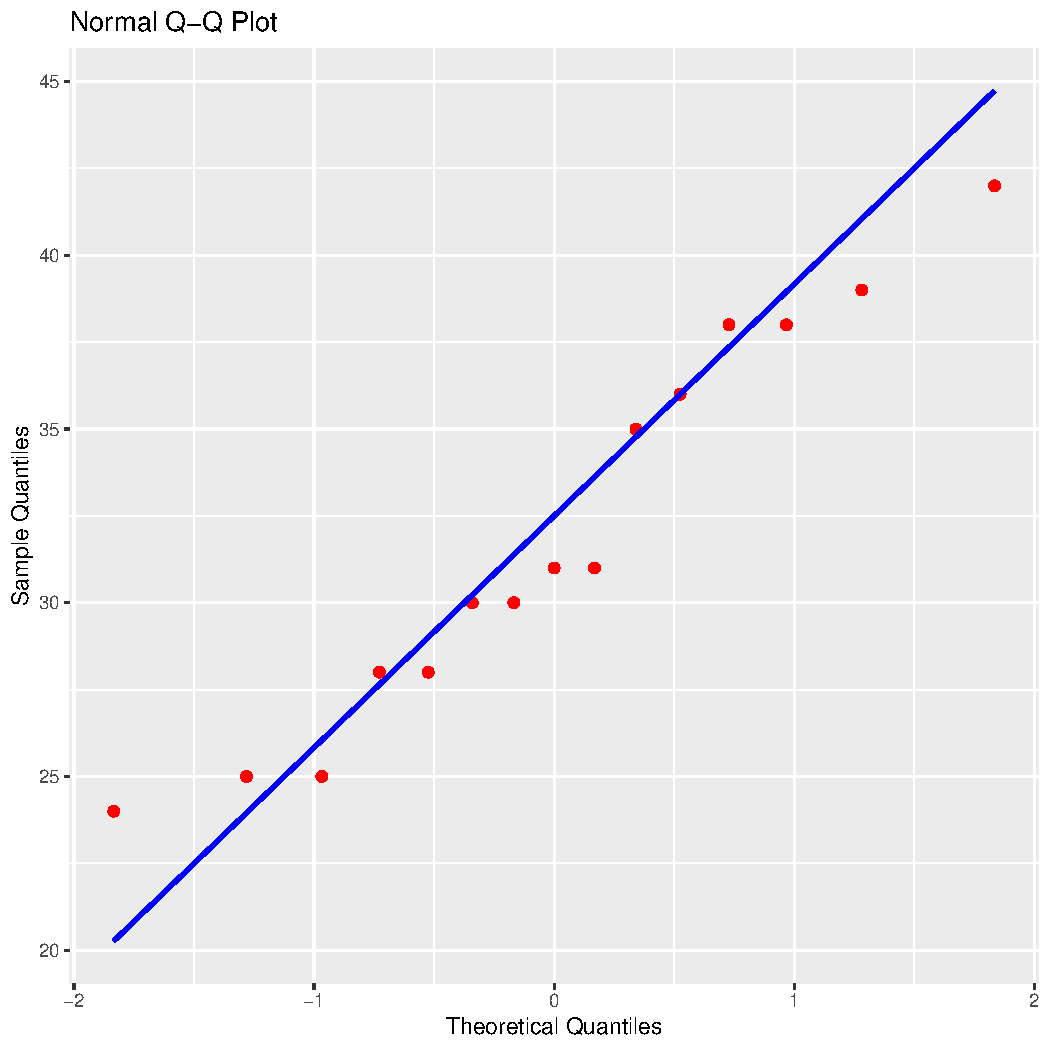
\includegraphics[width=\maxwidth]{figure/unnamed-chunk-4-1} 
\end{knitrout}
The points fit the line good. \\

$\bullet$ Checking Homoscedastic Variance

\begin{knitrout}\small
\definecolor{shadecolor}{rgb}{0.969, 0.969, 0.969}\color{fgcolor}\begin{kframe}
\begin{alltt}
\hlkwd{bartlett.test}\hldef{(speed} \hlopt{~} \hldef{machine,} \hlkwc{data} \hldef{= machine_data)}
\end{alltt}
\begin{verbatim}
## 
## 	Bartlett test of homogeneity of variances
## 
## data:  speed by machine
## Bartlett's K-squared = 1.8329, df = 2, p-value = 0.3999
\end{verbatim}
\end{kframe}
\end{knitrout}


A $p-$value of 0.3999448 results in failure of rejecting $H_0$ at $5\%$ level of significance that all the group variances are equal. This can also be verified by a box-plot.

\begin{knitrout}
\definecolor{shadecolor}{rgb}{0.969, 0.969, 0.969}\color{fgcolor}\begin{kframe}
\begin{alltt}
\hldef{machine_data} \hlopt
  \hlkwd{ggplot}\hldef{(}\hlkwd{aes}\hldef{(}\hlkwc{x} \hldef{= machine,} \hlkwc{y} \hldef{= speed))} \hlopt{+}
  \hlkwd{stat_boxplot}\hldef{(}\hlkwc{geom} \hldef{=} \hlsng{"errorbar"}\hldef{,} \hlkwc{linewidth} \hldef{=} \hlnum{1}\hldef{)} \hlopt{+}
  \hlkwd{geom_boxplot}\hldef{(}\hlkwc{fill} \hldef{=} \hlsng{"#eaf411"}\hldef{,} \hlkwc{linewidth} \hldef{=} \hlnum{1}\hldef{)} \hlopt{+}
  \hlkwd{stat_summary}\hldef{(}\hlkwc{fun} \hldef{= median,} \hlkwc{geom} \hldef{=} \hlsng{"point"}\hldef{,} \hlkwc{size} \hldef{=} \hlnum{3}\hldef{,} \hlkwc{col} \hldef{=} \hlsng{"red"}\hldef{)} \hlopt{+}
  \hlkwd{stat_summary}\hldef{(}\hlkwc{fun} \hldef{= median,} \hlkwc{geom} \hldef{=} \hlsng{"line"}\hldef{,} \hlkwd{aes}\hldef{(}\hlkwc{group} \hldef{=} \hlnum{1}\hldef{),} \hlkwc{linewidth} \hldef{=} \hlnum{1}\hldef{,} \hlkwc{col} \hldef{=} \hlsng{"blue"}\hldef{)} \hlopt{+}
  \hlkwd{labs}\hldef{(}\hlkwc{x} \hldef{=} \hlsng{"Machine"}\hldef{,} \hlkwc{y} \hldef{=} \hlsng{"Speed"}\hldef{,} \hlkwc{title} \hldef{=} \hlsng{"Boxplot of Speed ~ Machine"}\hldef{)}
\end{alltt}
\end{kframe}
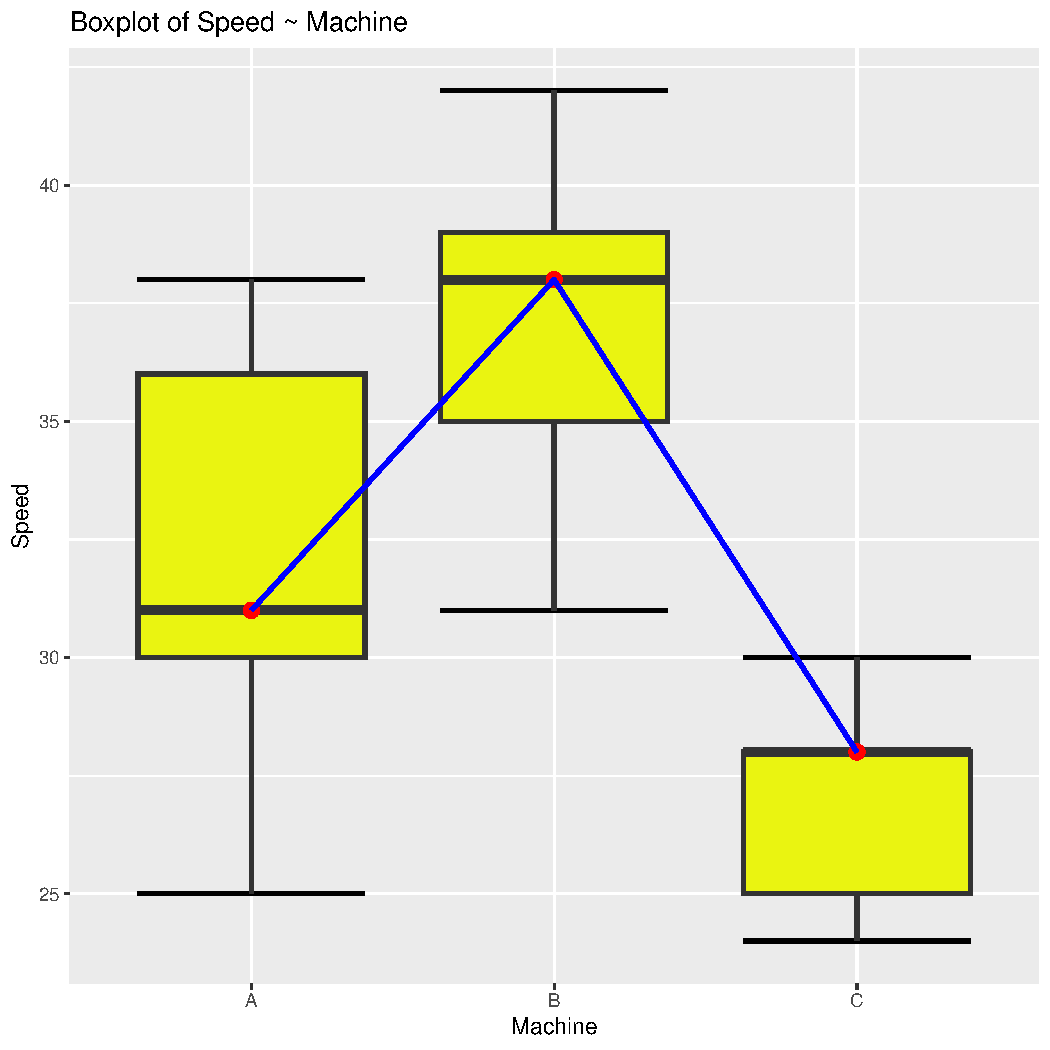
\includegraphics[width=\maxwidth]{figure/unnamed-chunk-6-1} 
\end{knitrout}

The spread of the boxes are more or less similar across groups. The line joining the group averages (here median) clearly shows that the sample machine average speeds differ a lot.

\newpage

\begin{knitrout}
\definecolor{shadecolor}{rgb}{0.969, 0.969, 0.969}\color{fgcolor}\begin{kframe}
\begin{alltt}
\hldef{machine_data_anova} \hlkwb{<-} \hlkwd{aov}\hldef{(speed} \hlopt{~} \hldef{machine,} \hlkwc{data} \hldef{= machine_data)}
\hlkwd{summary}\hldef{(machine_data_anova)}
\end{alltt}
\begin{verbatim}
##             Df Sum Sq Mean Sq F value  Pr(>F)   
## machine      2    250  125.00     7.5 0.00771 **
## Residuals   12    200   16.67                   
## ---
## Signif. codes:  0 '***' 0.001 '**' 0.01 '*' 0.05 '.' 0.1 ' ' 1
\end{verbatim}
\end{kframe}
\end{knitrout}

$p-$value corresponding to machine is 0.0077073 $< 0.05$. So we reject the null hypothesis of equality of mean machine speeds at $5\%$ level of significance and conclude that at least one of the machine has significantly different mean speed than others. \\

Now we shall do pairwise comparisons.
\begin{knitrout}
\definecolor{shadecolor}{rgb}{0.969, 0.969, 0.969}\color{fgcolor}\begin{kframe}
\begin{alltt}
\hlkwd{TukeyHSD}\hldef{(machine_data_anova,} \hlkwc{ordered} \hldef{=} \hlnum{TRUE}\hldef{)}
\end{alltt}
\begin{verbatim}
##   Tukey multiple comparisons of means
##     95% family-wise confidence level
##     factor levels have been ordered
## 
## Fit: aov(formula = speed ~ machine, data = machine_data)
## 
## $machine
##     diff       lwr      upr     p adj
## A-C    5 -1.888394 11.88839 0.1709498
## B-C   10  3.111606 16.88839 0.0058028
## B-A    5 -1.888394 11.88839 0.1709498
\end{verbatim}
\end{kframe}
\end{knitrout}

$p-$value corresponding to comparison of Machine $B$ and Machine $C$ is 0.0058028 $< 0.025$. So machine $B$ and $C$ are significantly different at $5\%$ level of significance. Other comparisons are not significant. So we conclude that machine $B$ is the best as it has the highest sample mean speed.

\end{document}
